% -*- TeX-master: "main"; fill-column: 72 -*-

\section{Resolving render information}
\label{apdx-mappings}

\subsection{Mapping line endings to curves}
\label{mapping}

In order to apply a line ending which is defined using only 2D coordinates onto a line which
has been defined using 3D coordinates, we need to define a mapping.
The first definition we make is that the origin of the line ending viewport is
mapped to the end of the line to which the line ending is applied.
If the \token{enable\-Rotational\-Mapping} attribute is set to \val{false}, the
line endings coordinate system is the same as the global coordinate system used to draw the layout,
only the origin is moved to that end of the line the line ending is applied to. If
the \token{enable\-Rotational\-Mapping} attribute is set to \val{true}, which is
the default, we define that the x,y-plane of the line endings viewport is mapped to the
plane that results from taking the unit vector of the slope of the line and the unit
vector that results from ortho-normalizing the slope vector and a second vector
that has no component along the z-axis. If the slope of the line has a positive component along the x-axis,
the ortho-normalized vector also has to have a positive component along the y-axis. In order to retain the
right handed coordinate system, the z-axis of the line endings coordinate system is perpendicular to the plane created by the other two vectors and has a positive component along the global coordinate systems z-axis.
Likewise if the slope has a negative component along the global coordinate systems x-axis, the y-component of the
ortho-normalized second vector has a negative component along the y-axis of the global coordinate system and to 
retain the right handed coordinate system, the third vector which is perpendicular to the plane made by the slope
and its ortho-normalized vector, has a positive component along the global coordinate systems z-axis. 

If the slope of the line points directly along the positive z-axis of the global coordinate system, the 
line endings coordinate system is mapped to the line ending by a -90 rotation around the y-axis of the 
line endings coordinate system and a translation of the origin of the line endings coordinate system to 
the end of the line. If the slope points directly down the negative z-axis, the line endings coordinate 
system has to be rotated by +90 around its y-axis before translation to the position of the curves end.   

This may all sound very complicated, but in the end, the calculations to be done are not difficult and straightforward. 

The mapping of arrowheads to line endings involves some transformations which we would like to illustrate with two examples.
The first example as depicted in \ref{fig:2ArrowHeadMapping} defines a straight line and a line ending which is to be applied
to the end of the line. The line ending specifies a bounding box with a size of $4\times4$ and a position of $P(-2,-2)$. 
The origin of the line ending is at $o(0.0,0.0,0.0)$ and the bounding box extends along the positive x- and y-axes.
The position of the bounding box is the offset by which the origin of the bounding box has to be translated from the endpoint of the curve.

\begin{figure}[!ht]
\begin{center}
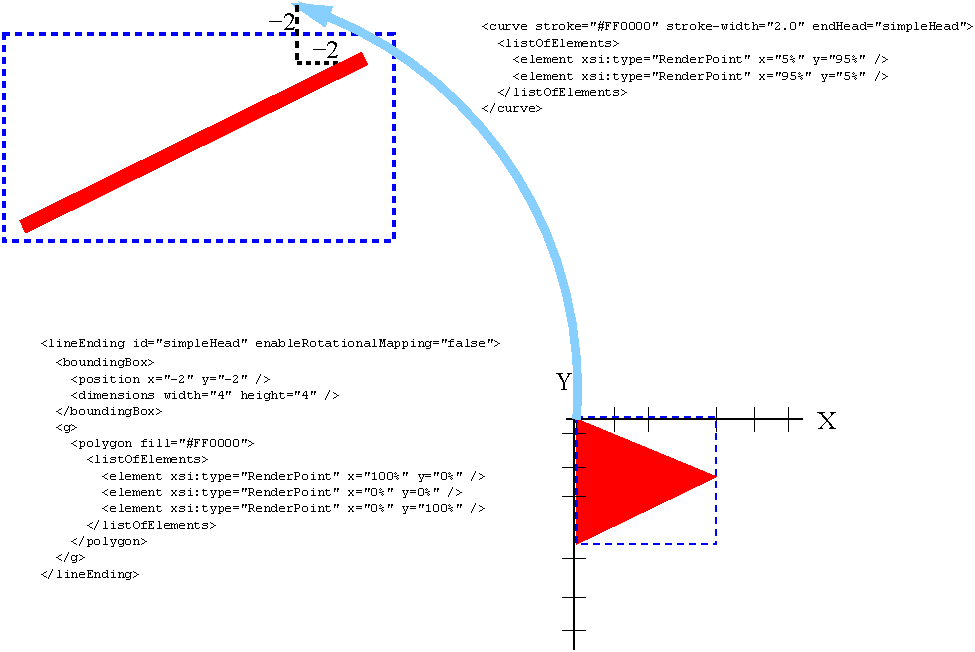
\includegraphics{figures/ArrowHeadMapping2.pdf}
\end{center}
\caption{Curve with arrow head and no rotational mapping} \label{fig:2ArrowHeadMapping}
\end{figure}

Since the arrow head in the first example explicitly disables rotation mapping by specifying \textbf{enableRotationalMapping=false}
in the definition of the line ending, the process of mapping the arrow head to the line is simply a matter of moving the origin of 
the line endings coordinate system to the end point of the line $E(ex,ey)$ plus the offset that is specified as the position $P(px,py,pz)$ of the line endings bounding box $F=E+P=(ex+px,ey+py,ez+pz)$. In our example the origin of the line endings coordinate system has to be moved 2 units up and two to the left of the and of the curve that the line ending is applied to.

The result of this operation is depicted in \ref{fig:3ArrowHeadMapping}.

\begin{figure}[!ht]
\begin{center}
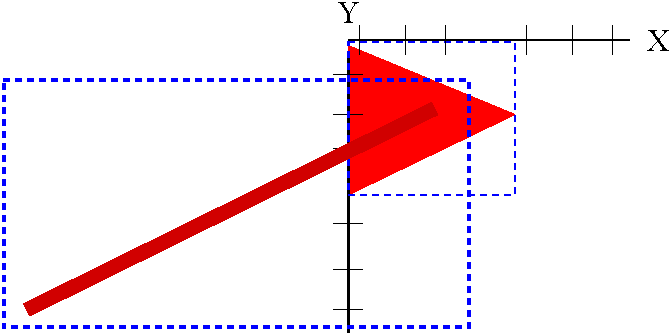
\includegraphics{figures/ArrowHeadMapping3.pdf}
\end{center}
\caption{Curve with mapped arrow head and no rotational mapping} \label{fig:3ArrowHeadMapping}
\end{figure}

The second example is very similar to the first example, only now, the rotational mapping for the arrow head is enabled.
This means that we now have to execute two steps in order to map the arrow head to the line ending.

First we need to rotate the arrow head so that the x-axis of the arrow heads coordinate system is aligned with the slope $s=\frac{dy}{dx}$ of the curve.

\begin{figure}[!ht]
\begin{center}
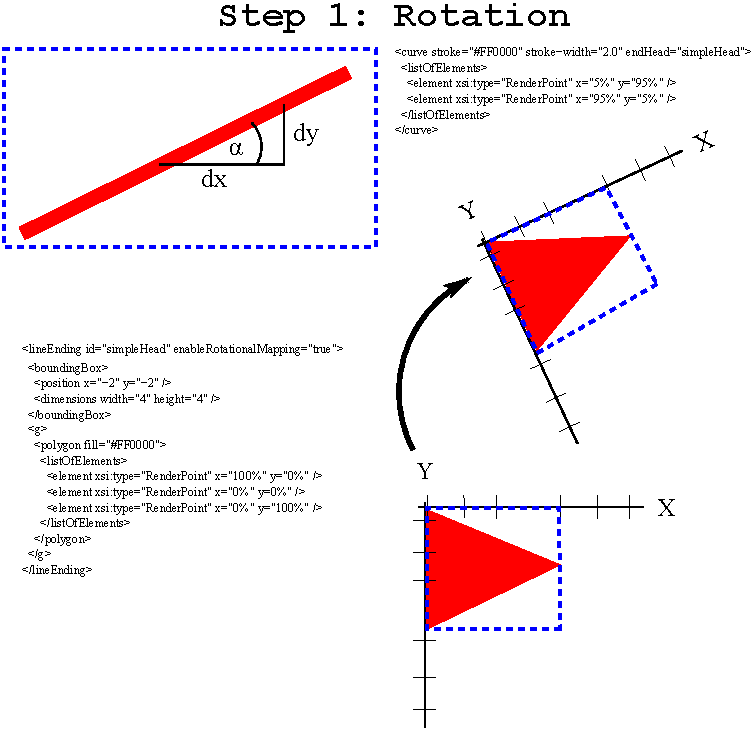
\includegraphics{figures/ArrowHeadMapping6.pdf}
\end{center}
\caption{Step 1: Rotation}
\label{ArrowHeadMapping6}
\end{figure}

The rotation of the arrow head involves the following steps:

\begin{enumerate}
\item{Calculate the normalized direction vector of the slope:\\
We first need to find the two points that determine the slope at the end of the line. One point is always the endpoint of 
the line ($E(ex,ey,ez)$). The second point depends on whether the last element of the line is a straight line or if it is
a Bézier element. If it is a Bézier element, the second point is the second base point of the Bézier element, if it is a 
straight line, it is either the preceding point or the endpoint of the preceding Bézier element. We call this second
point $S(sy,dy,sz)$.\\ The direction vector can be calculated as $v(vx,vy,vz)=(ex-sy.ey-sy,ez-sz)$. To normalize the vector
we have to calculate the length $l=\sqrt{vx^2+vy^2+vz^2}$ of the direction vector and divide all elements of $v$ by this
length: $v_n(v_{n}x,v_{n}y,v_{n}z)=(vx/l,vy/l,vz/l)$}.

\item{Calculate the normalized vector that is
\begin{enumerate}
\item{orthogonal to the direction vector of the line}
\item{located in the plane x- and y-axis}
\end{enumerate}
If the direction vector is parallel to the y-axis $(vx=0.0)$, the orthogonal vector $w$ is parallel to the x-axis ($w(vy,0,0)$).
For all other cases $w$ is $w(wx,wy,wz)=(-v_{n}y*v_{n}x,1-v_{n}y^2,-v_{n}y*v_{n}z)$.\\ Again, we have to normalize this
vector by dividing through its length $n=\sqrt{wx^2+wy^2+wz^2}$, which results in the normalized vector $w_n(w_{n}x,w_{n}y,w_{n}z)=(wx/n,wy/n,wz/n)$.
}
\item{Create the transformation matrix that converts the original coordinate system into the coordinate system
that is made up of the two calculated vectors. The transformation matrix that results from the two normalized vector that we calculated in the steps above
is 

\begin{center}
$m=\left(\begin{array}{cccc} v_{n}x & w_{n}x & 0.0 & 0.0\\ v_{n}y & w_{n}y & 0.0 & 0.0\\ v_{n}z & w_{n}z & 0.0 & 1.0 \end{array}\right)$
\end{center}
}


\end{enumerate}


The second step moves the origin of the arrow heads coordinate system to the endpoint of the line, which is exactly the same as we did in the first example.

\begin{figure}[!ht]
\begin{center}
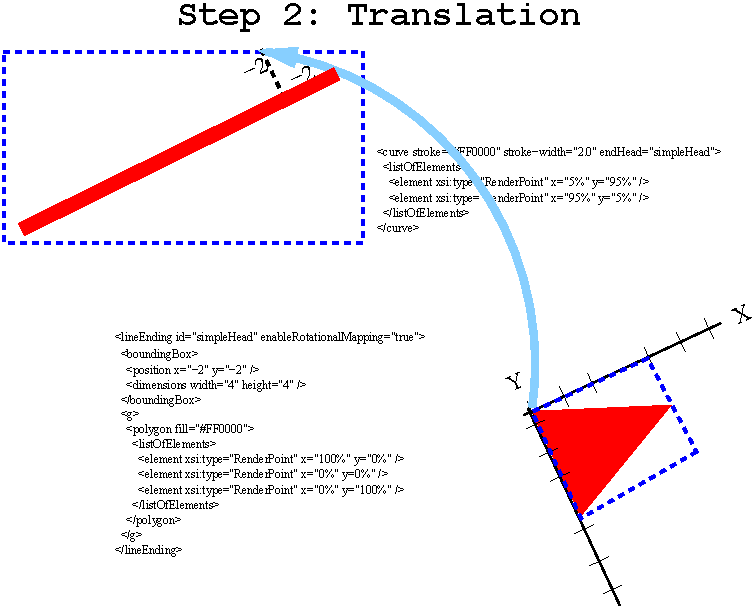
\includegraphics{figures/ArrowHeadMapping4.pdf}
\end{center}
\caption{Step 2: Translation}
\label{ArrowHeadMapping4}
\end{figure}

\begin{figure}[!ht]
\begin{center}
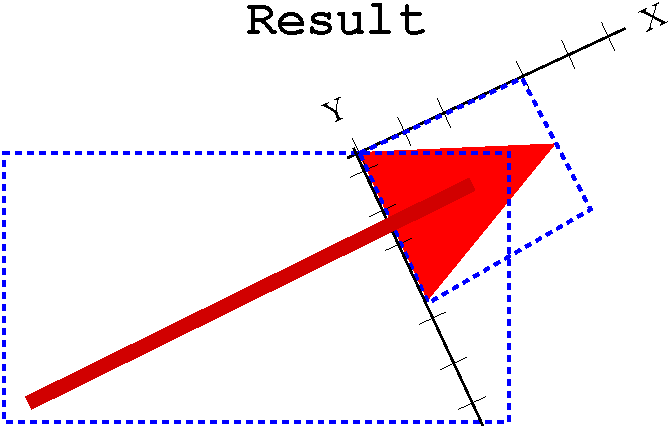
\includegraphics{figures/ArrowHeadMapping5.pdf}
\end{center}
\caption{Curve with mapped arrow head and rotational mapping}
\label{ArrowHeadMapping5}
\end{figure}

Mapping of an arrow head to the beginning of a curve is exactly the same as for the end of a curve, only the
direction of the line has to be reversed and in case of a cubic bezier, one has to use the first base point rather than the second base point. 

\subsection{Style resolution}
\label{style-res}

To resolve which style applies to a certain object, one 
should follow the rule that more specific style definitions take precedence 
over less specific ones and that if there are several styles with the same 
specificity, the first one encountered in the file is to be used. In essence,
this means that a program first has to search the local render information for 
a style that references the id of the object. If none is found, it searches for 
a style that mentions the role of the object. If it has one, see next section. 
If it does not find one, it searches for a style for the type of the object. 

If a render information references another render information object via its 
\token{reference\-Render\-Information} attribute, the program has to go through 
that one as well to see if a more specific render information is present there. 
If the chain of referenced \RenderInformation objects has been searched and no 
style has been found that fits, it is up to the program how the object is 
rendered. 

If several type-based styles are found 
that would fit, a style that applies to only one type takes precedence over a 
style that applies to several types.

If a program explicitly wants to define render information that 
states that some objects are not to be rendered at all, it has to define a 
style that does nothing, i.e., has no render information but applies to the 
objects that should not be rendered. 


\subsection{Role resolution}
\label{role-res}

This render extension explicitly provides means to write render information
that renders layout objects based on certain roles those render objects or their
corresponding model objects have. So far SBML models or layouts do not contain
such role information or only for a limited number of objects if one would
consider the role attribute of \class{SpeciesReferenceGlyph} objects to fall into this category.
Although there is currently no means to specify these roles, there are already
initiatives underway that try to complement SBML files with more biological
information based on ontologies.  

For the time being, we define an additional attribute called \token{objectRole} for all 
layout objects derived from \GraphicalObject including \GraphicalObject itself.
The attribute specifies a user defined role string. Render information including the same role string in its
\token{roleList} attribute applies to the object. This is only true if no more specific render information
takes precedence (see ``Style resolution'').
 
A specific style can reference one or more roles to which it applies. When a program tries to determine which style applies to a 
specific object it might have to determine the role of the object layout first. If the 
layout object itself has a role, this will be taken, otherwise if the layout object 
is associated with an object in the model, the program should get the role from 
the associated object. If none of them has a role, no role based style can be 
applied to the object.

\subsection{Style information for reaction glyphs and species reference glyphs}

When defining a style for a \class{ReactionGlyph} or \class{SpeciesReferenceGlyph} object, one 
has to distinguish between layout objects that only specify a bounding box for the 
object and those that specify a curve. In the case of a bounding box, it is necessary to 
define complete render information, whereas in the case of a curve, only 
certain attributes that determine certain aspects of how the 
curve should be drawn, e.g., its color. To resolve this conflict, the style for such an 
object has to define render information for both cases. The render information 
for the case of a bounding box is specified just like render information for 
any other object within a group. Render information for the case of a curve is 
defined by the appropriate attributes that are in effect in the outermost \RenderGroup 
object itself. Those attributes include \token{stroke}, \token{stroke-width} 
and \token{stroke-dasharray}. Additionally, \token{startHead} and \token{endHead} can be 
specified to define line endings for layout curve objects. If the group does not define 
one or more of these attributes, the default value is used (see also \sec{defaultvalues-class}).

\begin{figure}[!ht]
\begin{center}
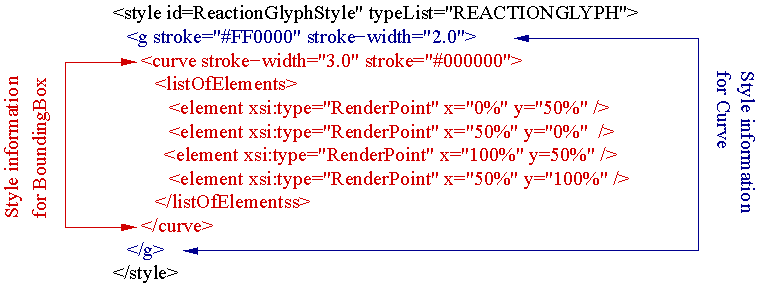
\includegraphics{figures/CurveAndBBStyle.pdf}
\end{center}
\caption{style with render information for objects with curve or bounding box}
\label{CurveAndBBStyle}
\end{figure}

\subsection{Style information for text glyphs}
Just as in the case of curves in {\class{ReactionGlyph}}s and {\class{SpeciesReferenceGlyph}}s,
{\class{TextGlyph}}s can be considered render information which is located
in the layout. A \class{TextGlyph} specifies the text to be rendered,
it therefore does not need additional render information in the form of
a \texttt{text} element. On the other hand, it needs render information in the form of font properties.
Just as for the \RenderCurve
object for {\class{ReactionGlyph}}s and {\class{SpeciesReferenceGlyph}}s, this render information is
taken from the font related attributes of the outermost group element of the
style that is used to render a \class{TextGlyph}. Any additional information within the
group is ignored. If the group does not specify any of the \token{font-family},
\token{font-size}, \token{font-weight}, \token{font-style}, 
\token{text-anchor} or \token{vtext-anchor} attributes, the default values are to be used.
